\chapter{Círculos armónicos por canción}\label{ap:circulos}

El cuaderno dibuja, para cada canción, un círculo armónico de 24 posiciones contadas desde la tónica. Reúne el perfil del
bajo, el de la voz aguda y el de las fundamentales, las transiciones entre fundamentales y el ritmo armónico. Son la
versión por canción, en disposición cromática, de la figura~\ref{fig:circulo}.

\begin{figure}[ht]
  \centering
  \begin{subfigure}{0.48\textwidth}\centering
    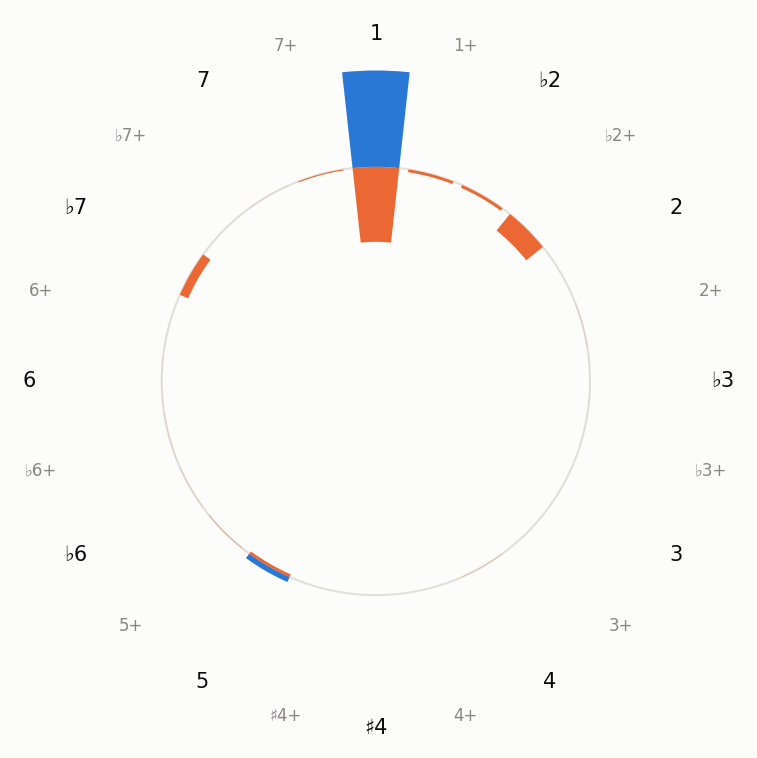
\includegraphics[width=\linewidth]{mata_zyklek_circulo_armonico.png}\caption{Mata Zyklek.}
  \end{subfigure}\hfill
  \begin{subfigure}{0.48\textwidth}\centering
    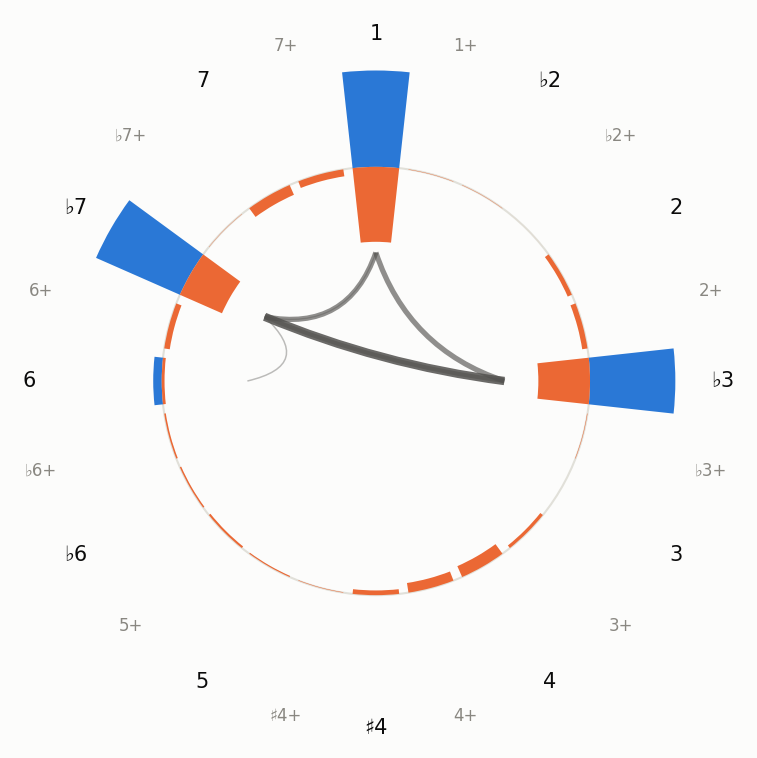
\includegraphics[width=\linewidth]{fabienk_circulo_armonico.png}\caption{Fabienk.}
  \end{subfigure}\\[0.6em]
  \begin{subfigure}{0.48\textwidth}\centering
    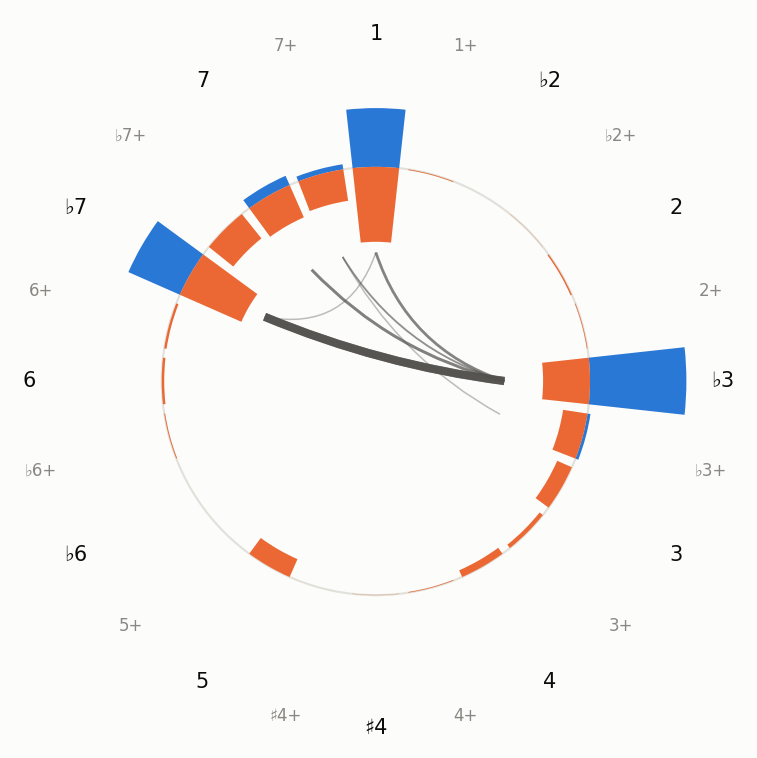
\includegraphics[width=\linewidth]{sarniezz_circulo_armonico.png}\caption{Sarniezz.}
  \end{subfigure}\hfill
  \begin{subfigure}{0.48\textwidth}\centering
    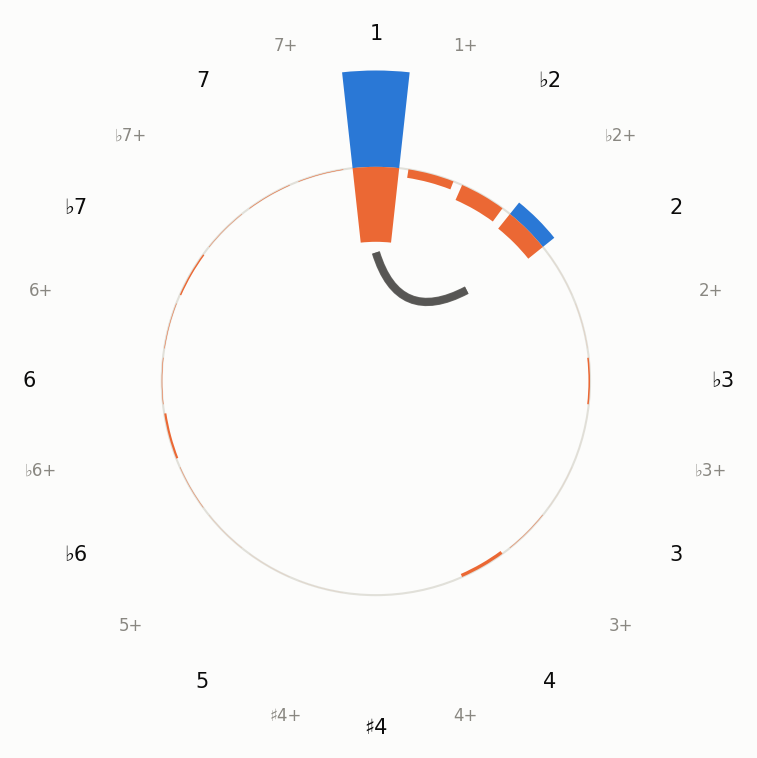
\includegraphics[width=\linewidth]{yor_zarad_circulo_armonico.png}\caption{Yor Zarad.}
  \end{subfigure}
  \caption{Círculos armónicos (I).}\label{fig:circulos1}
\end{figure}

\begin{figure}[ht]
  \centering
  \begin{subfigure}{0.48\textwidth}\centering
    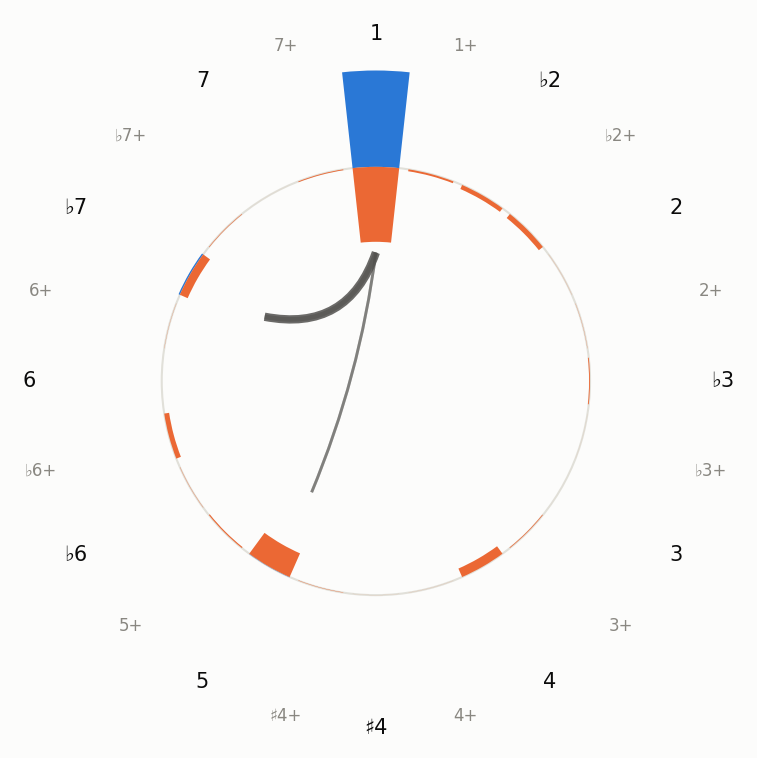
\includegraphics[width=\linewidth]{utzp_circulo_armonico.png}\caption{Utzp.}
  \end{subfigure}\hfill
  \begin{subfigure}{0.48\textwidth}\centering
    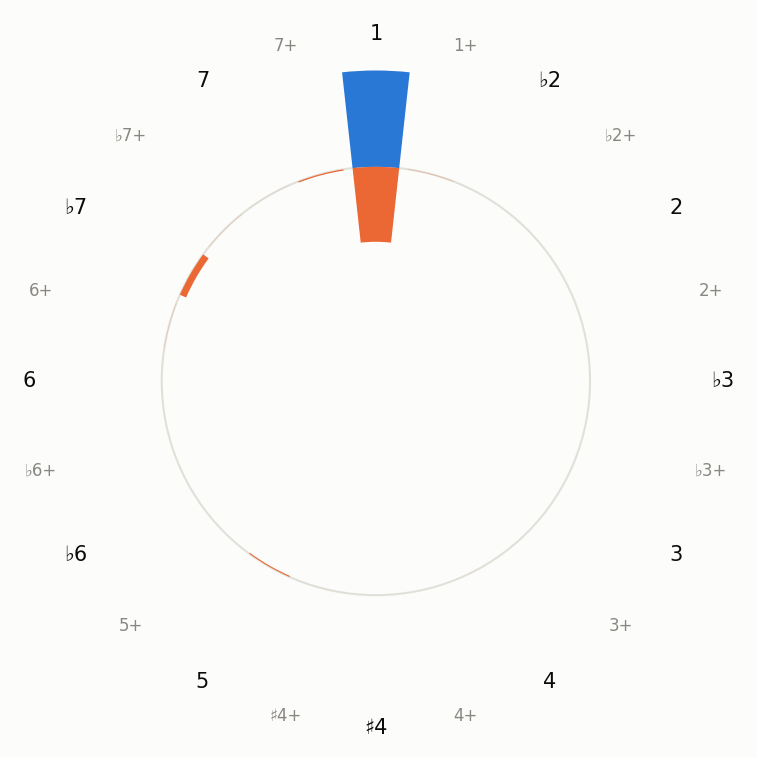
\includegraphics[width=\linewidth]{angor_circulo_armonico.png}\caption{Angor.}
  \end{subfigure}
  \caption{Círculos armónicos (II).}\label{fig:circulos2}
\end{figure}

\chapter{Glosario}\label{ap:glosario}

\section*{Altura y afinación}
\begin{description}[style=nextline,leftmargin=1.2em]
  \item[Cent] Centésima parte de un semitono temperado; la octava mide 1200 cents.
  \item[$q$-EDO] Sistema que divide la octava en $q$ partes iguales. 12-EDO es el temperamento usual; 24-EDO divide cada
  semitono en dos cuartos de tono de 50 cents.
  \item[Cuarto de tono] Intervalo de 50 cents. En este trabajo se escribe «+» sobre la nota o el grado (Sol+, \fl2+).
  \item[Clase de altura] Altura sin importar la octava; en 24-EDO hay 24 clases.
  \item[MIDI fraccionario] Número de nota continuo: $69 + 12\log_2(f/440)$. 52.5 es un cuarto de tono sobre Mi.
  \item[Campo] Cada una de las dos órbitas del ciclo de quintas en 24-EDO: grados regulares y grados en cuarto de tono.
  \item[Tercera neutra] Tercera de 350 cents, entre la menor y la mayor; solo existe con cuartos de tono.
  \item[Grado fijo] Nota de la escala que vuelve en cada vuelta del loop, a diferencia de un adorno de paso.
  \item[Inflexión] Cuarto de tono breve que llega o sale por un paso de cuarto de tono hacia un grado regular: un bend, un
  slide o una nota de paso.
  \item[Piso de ruido] Tiempo en cuartos de tono que la herramienta marca en música sin cuartos de tono (Primus, 9--13\,\%).
\end{description}

\section*{Señal y transcripción}
\begin{description}[style=nextline,leftmargin=1.2em]
  \item[Espectrograma] Energía de cada frecuencia en cada instante, calculada con la transformada de Fourier de tiempo
  corto.
  \item[Saliencia armónica] Evidencia de cada altura candidata, obtenida sumando la energía de sus armónicos.
  \item[pYIN] Estimador de la frecuencia fundamental de una sola voz \citep{mauch2014}.
  \item[Viterbi] Algoritmo de programación dinámica que elige la sucesión de estados de mayor puntaje.
  \item[MFCC] Coeficientes cepstrales en escala Mel: describen el timbre, no la nota.
  \item[Separación de fuentes] Extracción de la pista de cada instrumento a partir de la mezcla (Demucs, BS-RoFormer).
  \item[SDR] \emph{Signal-to-distortion ratio}: qué tan limpia sale una pista separada, en decibeles.
  \item[Looper] Dispositivo que graba una frase y la repite en bucle mientras se toca encima.
  \item[Ciclo] Tramo en que una voz repite un patrón con un periodo fijo; cada ciclo distinto recibe una letra.
  \item[Consenso entre vueltas] Promedio de la saliencia en los instantes equivalentes de vueltas vecinas del ciclo.
  \item[Piano roll] Gráfica con el tiempo en el eje horizontal y la altura en el vertical.
  \item[Tabroll] El piano roll de este trabajo: 24 filas por octava, compases y un acorde por compás, generado desde el
  audio.
\end{description}

\section*{Armonía}
\begin{description}[style=nextline,leftmargin=1.2em]
  \item[Fundamental] Nota que da nombre al acorde.
  \item[Calidad] Tipo de acorde según sus intervalos: quinta sola, menor, neutro, mayor, disminuido, aumentado, sus2 o
  sus4.
  \item[Centro] La nota de reposo de la canción; aquí se mide en tres partes (tiempo, bordes de vuelta y regresos).
  \item[Grado y cifrado] Posición de la fundamental respecto del centro, escrita en números romanos (I, \fl III, \fl VII,
  \fl II+).
  \item[Función] Papel del acorde según Riemann: tónica, subdominante o dominante; neutra para los grados en cuarto de tono.
  \item[Eje] Grupo de grados a distancia de tercera menor que comparten función, según Lendvai.
  \item[Pedal] Nota que se sostiene o se repite mientras la armonía se mueve encima.
  \item[Vaivén] Ida y vuelta repetida entre dos acordes.
  \item[Confianza $\kappa$] Qué tan segura está la herramienta del acorde de un compás; confiable si $\kappa \ge 0.5$.
  \item[Modo] Escala de siete grados con un centro (dórico, frigio, frigio dominante\dots).
\end{description}

\section*{Comparación y evaluación}
\begin{description}[style=nextline,leftmargin=1.2em]
  \item[Corpus] Colección de piezas de un estilo guardadas como notas o acordes.
  \item[Reparto de fundamentales] Fracción del tiempo que la canción pasa sobre cada grado.
  \item[Divergencia de Jensen-Shannon] Medida de diferencia entre dos repartos, de 0 (iguales) a 1 (nada en común).
  \item[Percentil de tipicidad] Porcentaje de piezas del corpus igual o más lejos que la canción: 50 es típica, 0 más rara
  que todas.
  \item[Bloque de rasgos] Conjunto de medidas de una dimensión: armonía, escala, cuartos de tono o metro.
  \item[Sin vecino] Ningún corpus llega al percentil 5 en un bloque.
  \item[Calibración] Aplicar el método a piezas cuya respuesta se conoce para medir cuánto se equivoca.
  \item[Medida F] Media armónica de la precisión y la exhaustividad de una transcripción.
  \item[Referencia corregida de oído] Partitura verificada por el autor contra fragmentos de la grabación.
  \item[Arbitraje a ciegas] Escucha de versiones en orden al azar, sin saber cuál es de la partitura y cuál de la
  herramienta.
  \item[Semilla fija] Valor que fija el azar del programa para que cada corrida dé lo mismo.
  \item[Huella SHA-256] Código de 64 caracteres que identifica un archivo y cambia si el archivo cambia \citep{nist2015}.
\end{description}
